%!TEX root = main.tex

\section{Continuous training on edge compute}
\label{sec:background}

%We explain the edge computing setup for video analytics (\S\ref{subsec:edge}) and motivate continuous training of video DNNs (\S\ref{subsec:continuous}).


\subsection{Edge Computing for Video Analytics}
\label{subsec:edge}

% edge computing setup: managed edge outposts & their specs, processing videos in a building or campus; typical video streams/edge
Video analytics deployments commonly analyze videos on edge servers placed on-premise (e.g., from AWS \cite{aws-outposts} or Azure \cite{azure-ase}). % or embedded compute with camera (e.g., \cite{DBLP:conf/mobisys/NaderipariziZPP17, DBLP:conf/edge/WangFCGBPYS18}).
%These include private servers that are managed by the enterprises themselves or rented from cloud providers \cite{aws-outposts, azure-ase}. 
%, managed edge boxes rented from cloud providers, or  %(who also update \& maintain these boxes) 
%Computation on the edge servers is typically using containers that are orchestrated by frameworks like Kubernetes \cite{kubernetes}. 
%%%Due to cost and energy constraints, compute efficiency is one of the key design goals of edge computing. 
%A recent study %of video analytics edge deployments 
%concludes that the setup of edge {\em servers} are more popular than cameras with compute on-board %due to ease of maintenance and amortization of cost when analyzing multiple video streams %\cite{getmobile}. %Video analytics applications are usually composed of a pipeline of one or more containers that work together \cite{rocket-github}. 
A typical edge server supports tens of video streams \cite{videoedge}, e.g., on the cameras in a building, with customized models for each stream \cite{rocket-github} (see Figure \ref{fig:edge}).%, that execute in parallel using video analytics pipelines \cite{rocket-github}. 
% bandwidth and privacy reasons; point to prior work
Video analytics applications adopt edge computing for the following reasons %of limited network bandwidth to the cloud, unreliability of the network, and privacy of the video content 
\cite{getmobile, edgevideo-1, ieee-computer}. 

$1)$ Edge deployments are often in locations where the {\em uplink network to the cloud is expensive} for shipping continuous video streams, %that cannot support continuous upload of video streams to the cloud for processing, 
e.g., in oil rigs with expensive satellite network or smart cars with data-limited cellular network. %, where the costs grow with the volume of data transfer. 
\footnote{The uplinks of LTE cellular or satellite links is $3-10$Mb/s \cite{39-getmobile, 57-getmobile}, which can only support a couple of $1080$p 30 fps HD video streams whereas a typical deployment has many more cameras \cite{getmobile}.}

$2)$ Network links out of the edge locations experience {\em outages} \cite{20-getmobile, getmobile}. % and assuming reliable connectivity to the cloud risks disrupting business operations \cite{37-getmobile}. 
Edge compute provides robustness against disconnection to the cloud \cite{chick-fill} and prevents disruptions \cite{37-getmobile}. 

$3)$ Videos often contain {\em sensitive and private data} that users do not want sent to the cloud (e.g., many EU cities legally mandate that traffic videos be processed on-premise \cite{sweden-data, azure-data}). % Overall, {\em edge deployments for video analytics is cost-effective, robust, and private}, as has been observed by several prior works \cite{edge, compute, references}. 
%\ion{Can we have some numbers about the the available bandwidth and some data about network reliability of the edge servers?}
%\subsection{Continuous Training}

 \begin{figure}[t!]
     \centering
     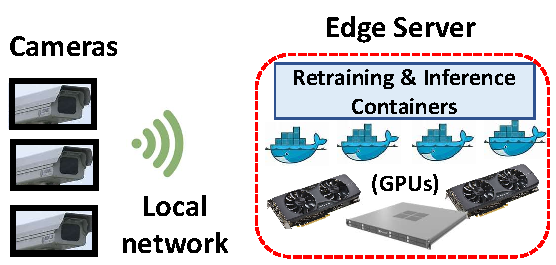
\includegraphics[width=0.6\columnwidth]{ekya/figures/xxx_cropped.pdf}
     \caption{\bf\small Cameras connect to the edge server, with consumer-grade GPUs for DNN inference and retraining containers.%. We propose extending the workload to include continuous retraining of DNNs.
     }
     \label{fig:edge}
 \end{figure}

Thus, due to reasons of network cost and video privacy, it is preferred to run both inference and retraining on the edge compute device itself without relying on the cloud. In fact, with bandwidths typical in edge deployments, cloud-based solutions are slower and result in lower accuracies (\S\ref{subsec:eval-alternate}).

\subsection{Compressed DNN Models and Data drift}
\label{subsec:continuous}

Advances in computer vision research have led to high-accuracy DNN models that %surpass human-level accuracy on general images and videos. These DNN models 
achieve high accuracy with a large number of weights, deep architectures, and copious training data. While highly accurate, using these heavy and general DNNs for video analytics is both expensive and slow \cite{noscope, DBLP:conf/osdi/HsiehABVBPGM18}, which make them unfit for resource-constrained edge computing. The most common approach to addressing the resource constraints on the edge is to train and deploy \emph{specialized and compressed} DNNs \cite{compression-4, compression-5, compression-6, compression-17, compression-18, compression-19}, which consist of far fewer weights and shallower architectures. \revtext{For instance, Microsoft's edge video analytics platform ~\cite{rocket-blog} uses a compressed DNN (TinyYOLO~\cite{redmon2018yolov3}) for efficiency. Similarly, Google released Learn2Compress\cite{learn2compress} for edge devices to automate the generation of compressed models from proprietary models.} These compressed DNNs are trained to only recognize the limited objects and scenes specific to each video stream. In other words, to maintain high accuracy, they forego generality for improved compute efficiency \cite{noscope, DBLP:conf/osdi/HsiehABVBPGM18, mullapudi2019}. 

% use cases - connected smart cars, indexing on iphone, even stationary traffic cameras
%Advances in DNN efficiency, e.g., using model compression \cite{compression-4, compression-5, compression-6, compression-17, compression-18, compression-19}, have enabled the deployment of DNN models on resource-constrained edge servers. Efficient edge models drive video analytics applications in modern cars, urban mobility traffic control, and enterprise campuses \cite{bellevue-report}. %Video analytics in smart cars already provide safety assist features (e.g., lane drift alerts) and many more such features are expected in the near future \cite{smart-cars}. Camera streams in enterprise buildings are analyzed for security applications as well as for ubiquitous sensing applications, e.g., face recognition to authenticate building access \cite{smart-buildings}. %Mobile devices use DNN object classifiers to generate ``tags'' for the pictures and videos clicked by users, thus enabling search by keywords (e.g., find pictures with a party hat) \cite{iphone-indexing}. 
%\junchen{this para could be a good fit to a new subsection of ``DNN deployed at the edge''?}
%\junchen{i like the idea of starting with data drift, though maybe we should motivate why data drift is so damaging in the first place? }

%\begin{figure}[t!]
%  \centering
%  \begin{subfigure}[t]{0.5\linewidth}
%    \centering
%    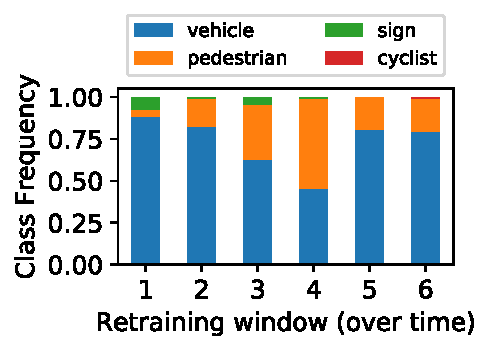
\includegraphics[width=\linewidth]{ekya/ekya/figures/motivation/incr_learn_motivation/motivation_waymo_distchange_classdist.pdf} 
%    \caption{\small Class distribution}
%    \label{fig:class-distrib-motivation}
%  \end{subfigure}
%  ~~~
%  \begin{subfigure}[t]{0.5\linewidth}
%    \centering
%    % 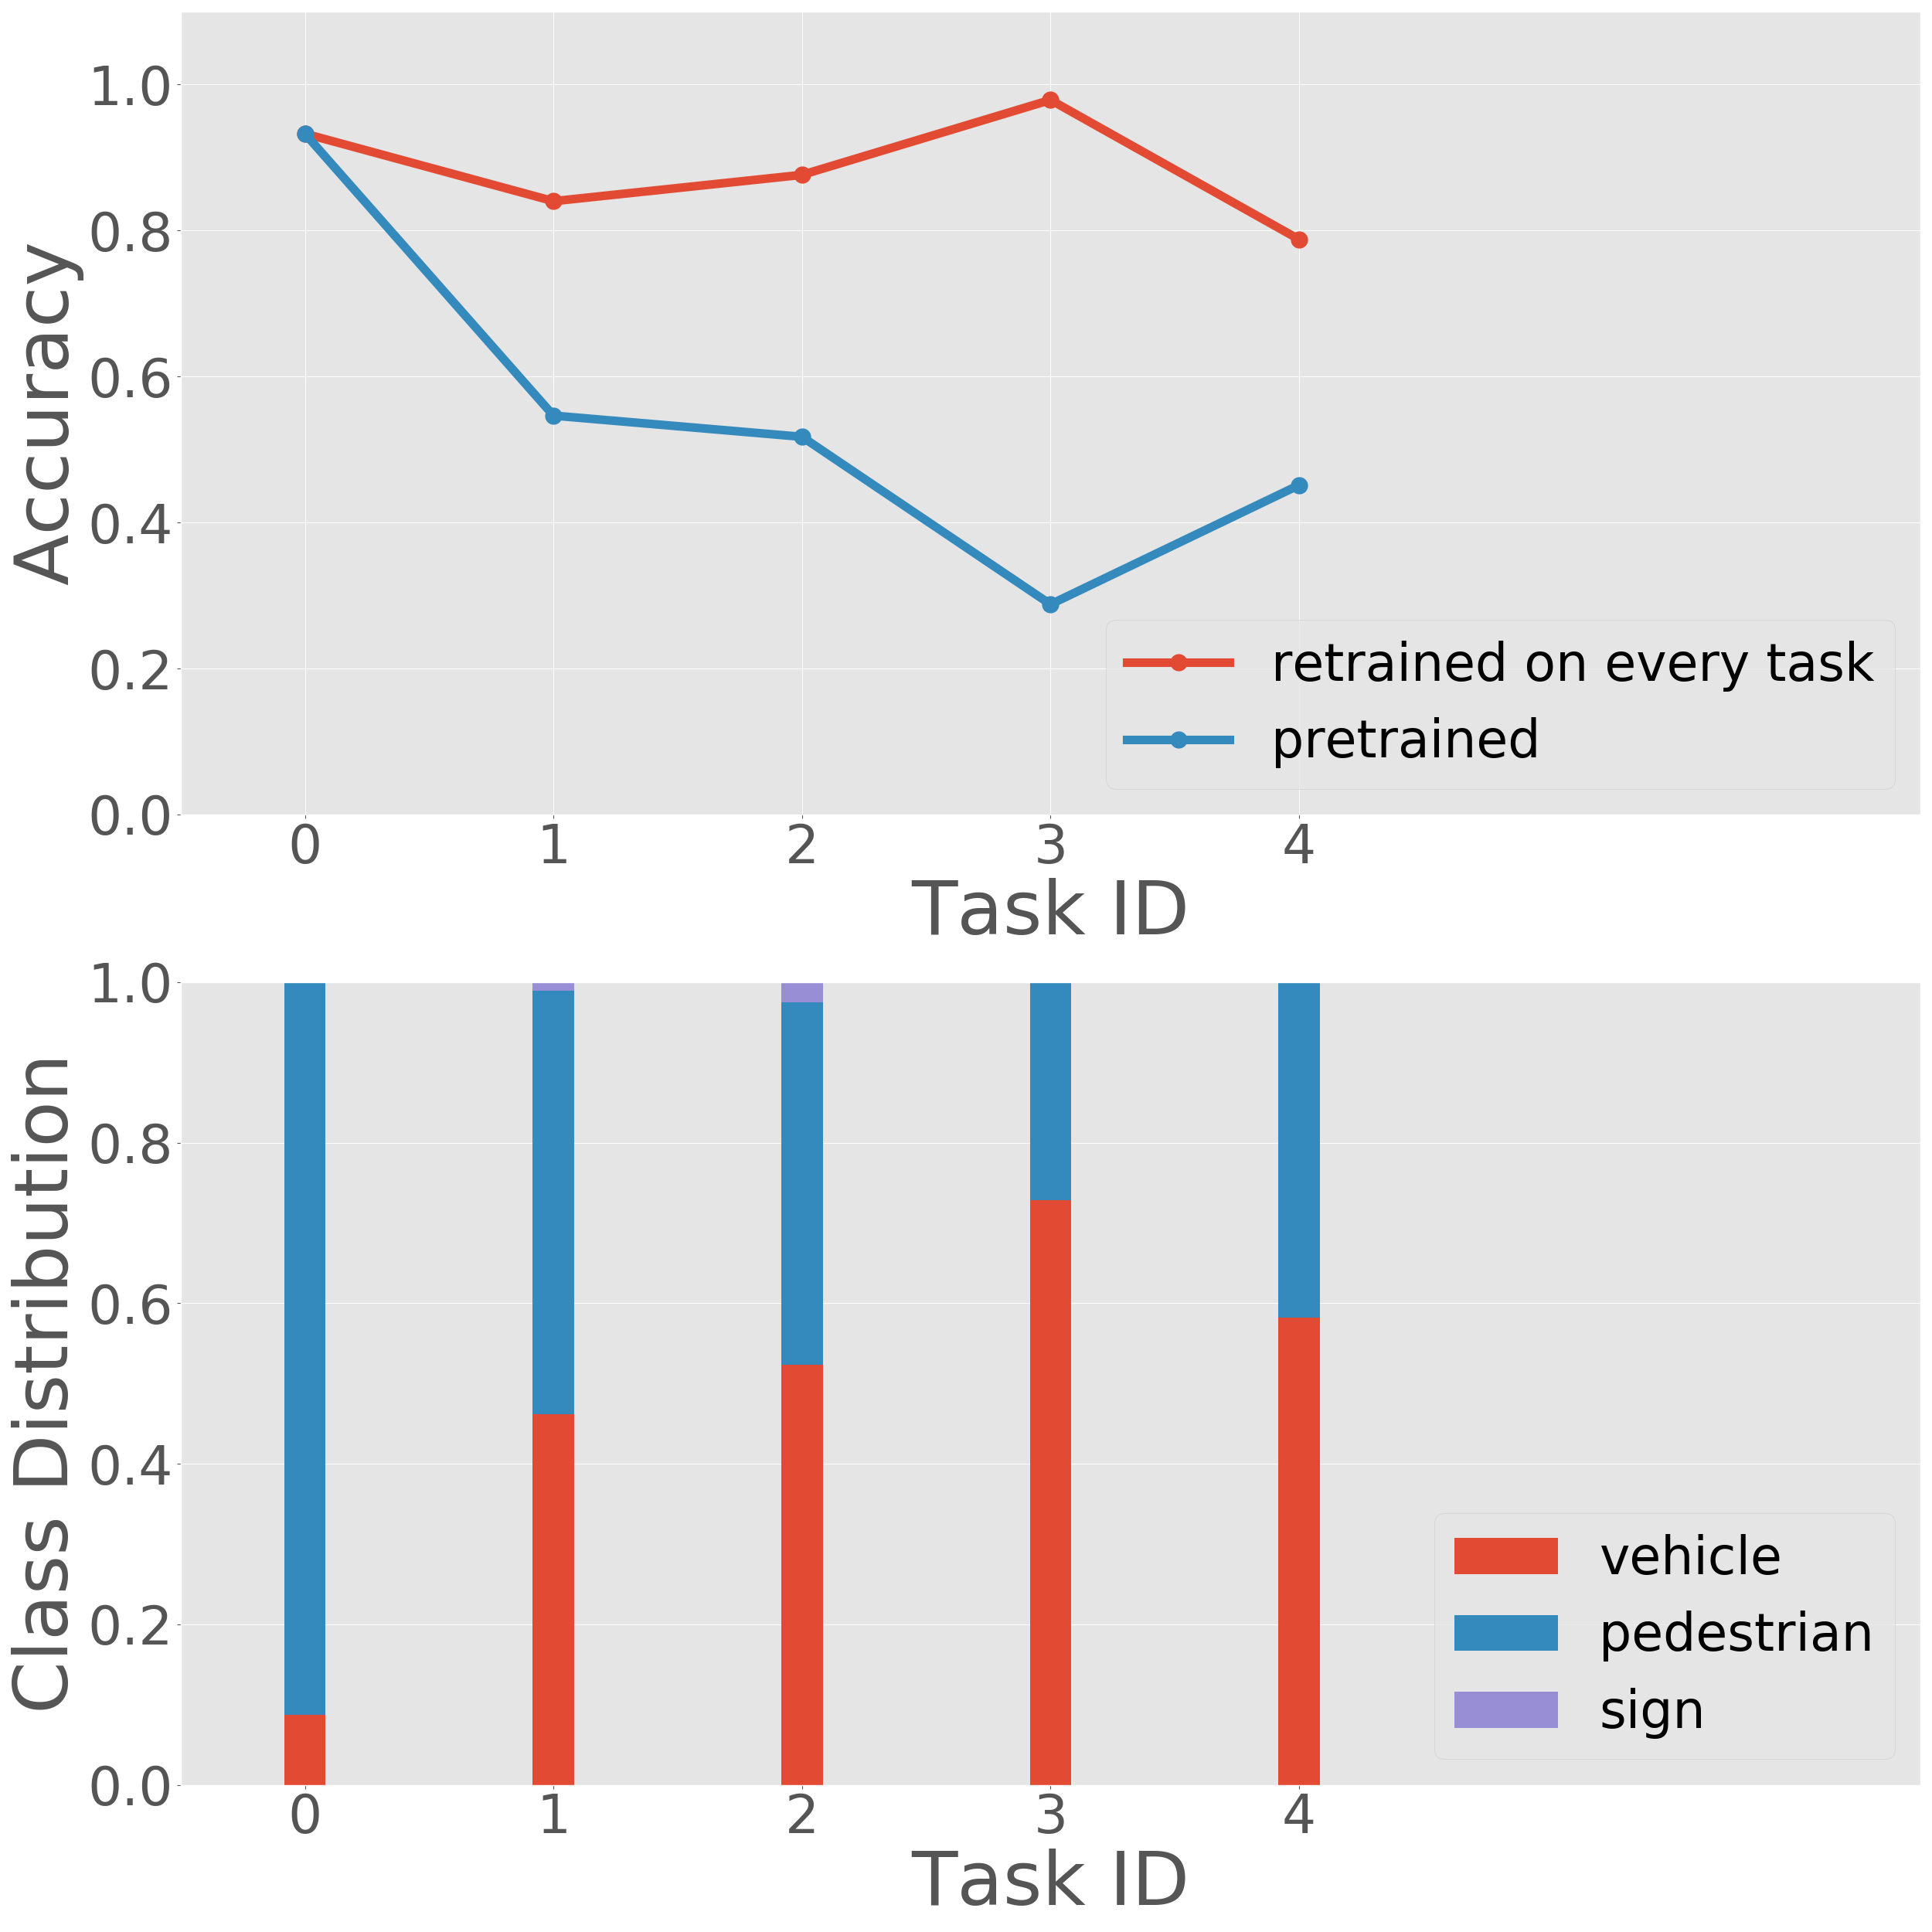
\includegraphics[width=\linewidth]{ekya/figures/motivation/Class_Incrementality/class_distribution_change_sf_27.png}
%    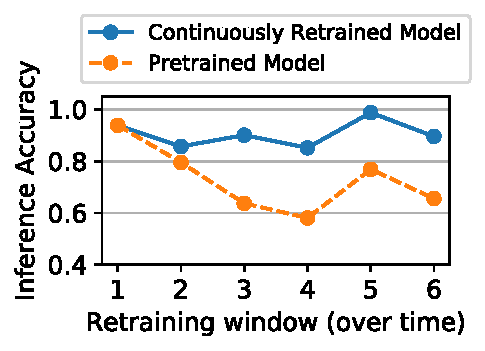
\includegraphics[width=\linewidth]{ekya/figures/motivation/incr_learn_motivation/motivation_waymo_distchange_acc.pdf}
%     \caption{\small Accuracy}
%    \label{fig:class-distrib-motivation-acc}
%  \end{subfigure}
%  \caption{\bf\small Impact of changing class distribution (left) on model accuracy in the Waymo data. Continuous learning results in higher and steady accuracy over time (right). \kh{Update the figures to include the one trained with first half of the tasks}}
%  \label{fig:waymo-motivation-distrib}
%\end{figure}


\noindent{\bf Data drift.} As specialized edge DNNs have shallower architectures than general DNNs, they can only memorize limited amount of object appearances, object classes, and scenes. As a result, specialized edge DNNs are particularly vulnerable to {\em data drift} \cite{datadrift-7, datadrift-8, datadrift-a, datadrift-b}, where live video data diverges significantly from the initial training data. For example, variations in the object pose, scene density (e.g. rush hours), and lighting (e.g., sunny vs. rainy days) over time make it difficult for traffic cameras to accurately identify the objects of interest (cars, bicycles, road signs). Cameras in modern cars observe vastly varying scenes (e.g., building types, crowd sizes) as they move through different neighborhoods and cities. Further, the {\em distribution} of the objects change over time, which reduces the edge model's accuracy \cite{distribution-20, distribution-21}. Due to their ability to memorize limited amount of object variations, edge DNNs have to be continuously updated with recent data and changing object distributions to maintain a high accuracy.  %Finally, newer object classes may appear (e.g., segway scooters) which may not have been available in the initial training data \cite{incremental-24, icarl-14}.  

%\vspace{-.05in}\subsubsection{\bf Data drift.} %While model compression has considerably increased the inference efficiency of DNN models, it also results in their having lower ``capacity'' to learn from their training data. 
%While compressed models are initially trained on representative data, when they are out in the field, they suffer from {\em data drift} \cite{datadrift-7, datadrift-8, datadrift-a, datadrift-b}. Data drift refers to the live video data diverging significantly from the initial training data. For example, traffic cameras encounter many variations in the angles of objects, scene density, and lighting over time, thus making it difficult to accurately identify the objects of interest (cars, bicycles, road signs).  
%Cameras in modern cars observe vastly varying scenes (e.g., building colors, crowd sizes) as they move through different neighborhoods and cities. %\ion{Are we considering cameras in slefdriving cars? If yes, I'm not sure about it. First, cars can have very powerful processors. Second, I don't think that we can easily sell the point about degrading inference to do the training in such a mission critical app (just add a second processor for inference). Third, not sure we want to deploy a model in a self-driving car without careful validation.} 


%The problem of data drift is exacerbated in compressed models. Compression of DNNs makes them efficient in their compute and memory demands, and facilitates their deployment on resource-constrained edge servers. However, smaller DNNs can memorize less due to their relatively limited capacity. In other words, their efficiency comes at the expense of generalizability to the data distributions of live inference videos that are different than their training data \cite{compressiondrift-22, compressiondrift-23, efficientnet-3}. %It is generally difficult to provide an exhaustive training dataset with enough samples to cover all possible variations.
%It is difficult and often intractable to provide an exhaustive training dataset with enough samples to cover all possible variations, especially in open real-world deployments. 

%\ga{Model capacity drops due to compression?} \junchen{to Ganesh's comment on compression vs. capacity: totally agree this is what any (knowledgeable) reviewer may wonder as well. i believe there {\em is} a fundamental tradeoff between capacity (how much to compress) and generalizability (robustness to data drift).maybe just cite the ECCV paper Romil found and ask Nikolas for more.} \ys{+1 on this point. The large the model is, the higher capacity it has. However, a large model not only requires a huge amount of data and time for training, but also leads to a higher runtime cost (memory, latency etc.) during inference. Hence, an alternative of having a large well-trained model is to maintain a localized cheaper model, and retrain it on demand. }

\noindent{\bf Continuous training.} The preferred approach, that has gained significant attention, is for edge DNNs to {\em continuously learn} as they incrementally observe new samples over time \cite{incremental-13, icarl-14, incremental-15}. %while not fully forgetting the learnings from old samples. 
The high temporal locality of videos allows the edge DNNs to focus their learning on the most recent object appearances and object classes \cite{DBLP:conf/cvpr/ShenHPK17, mullapudi2019}.  
%Incremental learning techniques %retain snapshots of history for the retraining (not the entire historical dataset) and  avoid {\em catastrophic forgetting} of the learnings on historical data \cite{datadrift-8} even as they learn from new data. 
%In \name, we use a modified version of iCaRL \cite{icarl-14} though our techniques are generally applicable.
In \name, we use a modified version of iCaRL\cite{icarl-14} learning algorithm to on-board new classes, as well as adapt to the changing characteristics of the existing classes. %We also tune the balance distillation and cross-entropy losses. 
%We use the iCaRL \cite{icarl-14} incremental learning algorithm for our experiments though the techniques in our work are generally applicable.
%In our solution, 
Since manual labeling is not feasible for continuous training systems on the edge, \revtext{the labels for the retraining are obtained from a ``golden model'' - a highly accurate (87\% and 84\% accuracy on Cityscapes and Waymo datasets, respectively) but expensive model (deeper architecture with large number of weights)}. The golden model cannot keep up with inference on the live videos and we use it to label only a small fraction of the videos in the retraining window. %\revtext{We then use these labels from the golden model to train compressed models.} 
Our approach is essentially that of supervising a low-cost ``student'' model with a high-cost ``teacher'' model (or knowledge distillation \cite{44873}), and this has been broadly applied in computer vision literature \cite{incremental-13, mullapudi2019, incremental-15, distribution-20}. %The use of a golden model for labeling is consistent with prior work in computer vision literature \cite{incremental-13, mullapudi2019, incremental-15, distribution-20}. 


% data drift; class incremental; waymo graphs; app-level impact
\subsection{Accuracy benefits of continuous learning}
\label{subsec:continuous-measurement}

\begin{figure}[t!]
  \centering
  % Accuracy figure
  % Class distribution figure
  \begin{subfigure}[t]{0.48\linewidth}
    \centering
    % 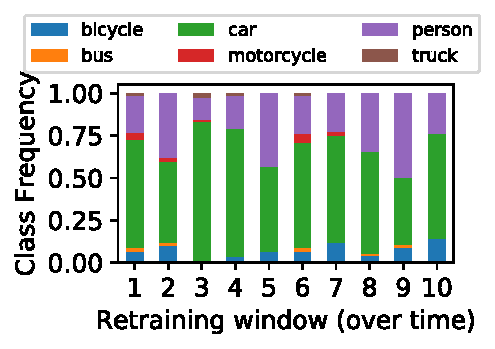
\includegraphics[width=\linewidth]{ekya/figures/motivation/incr_learn_motivation/motivation_jena_classdist.pdf}
    % 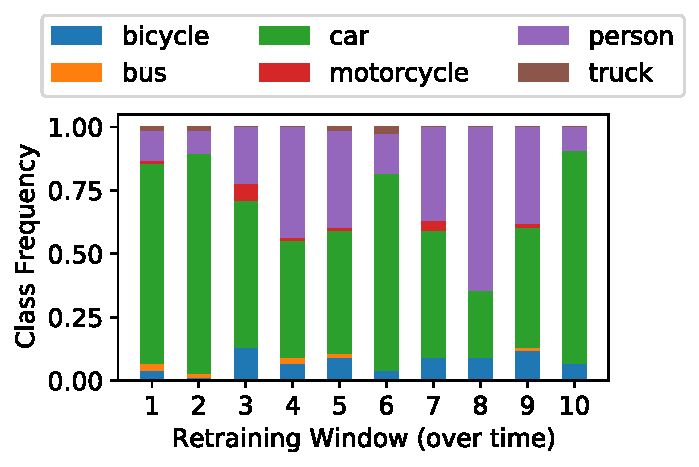
\includegraphics[width=\linewidth]{ekya/figures/motivation/incr_learn_motivation/motivation_cityscapes_jena_classdist.pdf}
    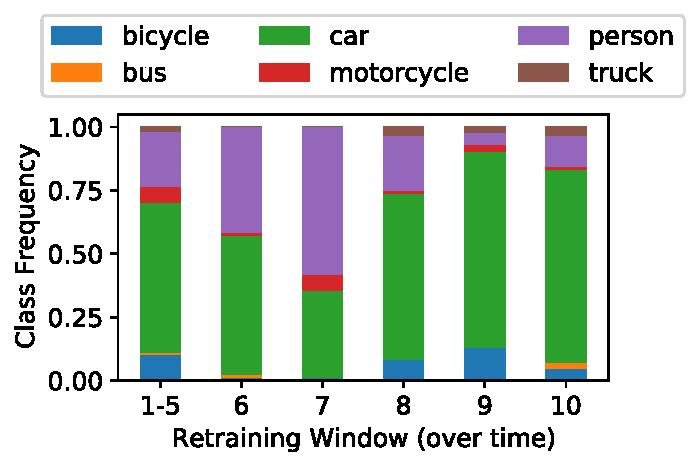
\includegraphics[width=\linewidth]{ekya/figures/motivation/incr_learn_motivation/motivation_cityscapes_zurich_classdist.pdf}
    \caption{\small Class Distribution}
    \label{fig:jena-classdist}
  \end{subfigure}
    ~~
  \begin{subfigure}[t]{0.48\linewidth}
    \centering
    % 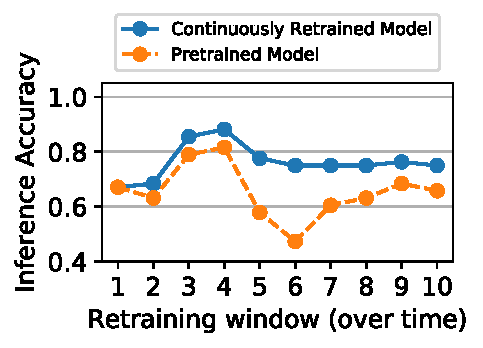
\includegraphics[width=\linewidth]{ekya/figures/motivation/incr_learn_motivation/motivation_jena_acc.pdf}
    % 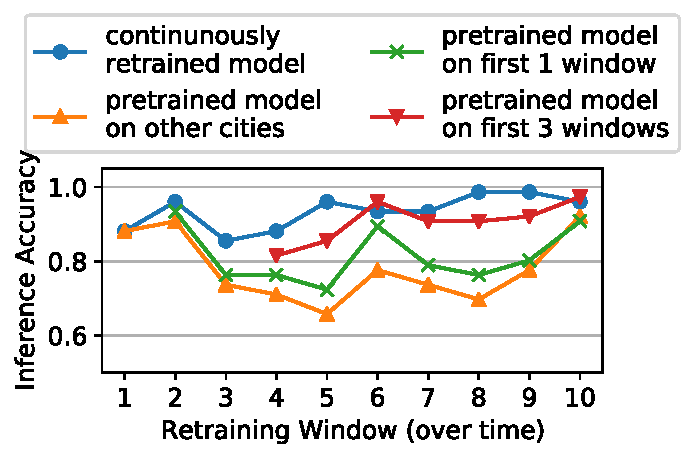
\includegraphics[width=\linewidth]{ekya/figures/motivation/incr_learn_motivation/motivation_cityscapes_jena_accuracy.pdf}
    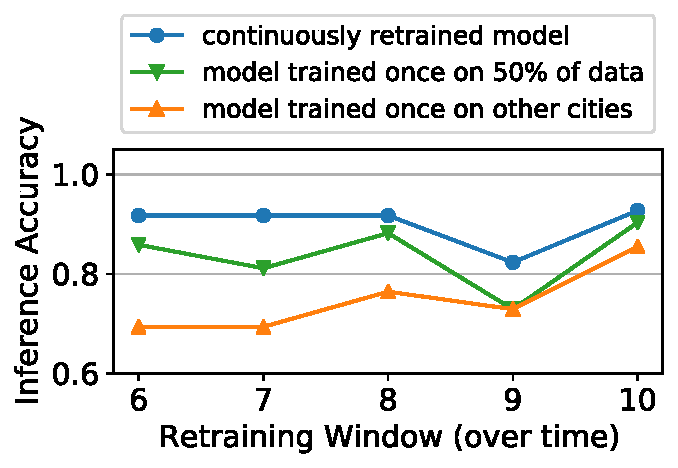
\includegraphics[width=\linewidth]{ekya/figures/motivation/incr_learn_motivation/new_motivation_cityscapes_zurich_accuracy.pdf}
    
    
    \caption{\small Accuracy}
    \label{fig:jena-motivation}
  \end{subfigure}
    \hspace*{\fill}
  ~~
  % Sample Image Task 1
  \begin{subfigure}[t]{0.46\linewidth}
    \centering
    % 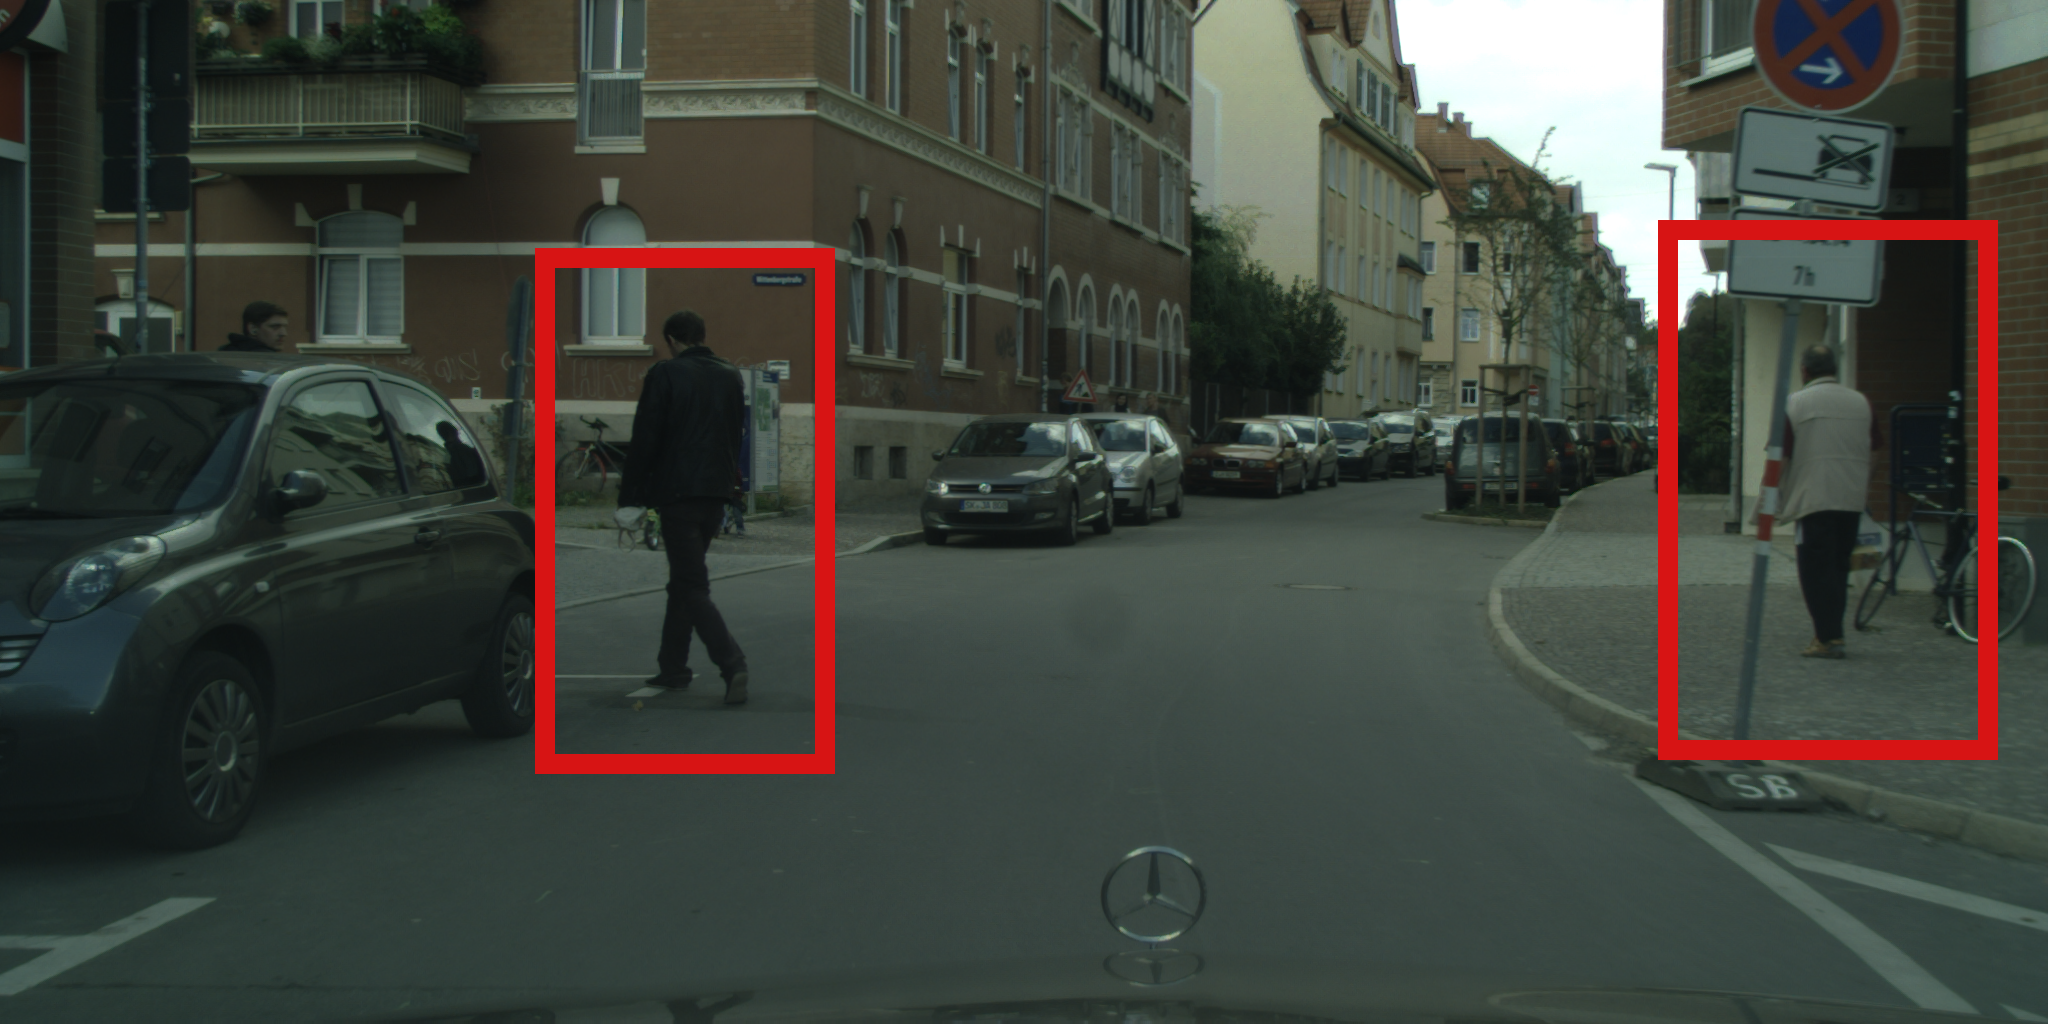
\includegraphics[width=\linewidth]{ekya/figures/motivation/incr_learn_motivation/t1_marked.png}
    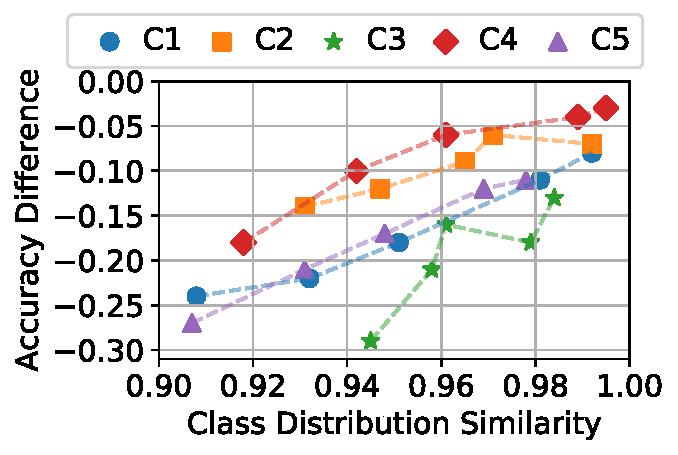
\includegraphics[width=\linewidth]{ekya/figures/motivation/incr_learn_motivation/motivation_datadrift_vs_acc.pdf}
     \caption{\small Accuracy vs data drift}
    \label{fig:acc-datadrift}
  \end{subfigure}
  ~~
  % Sample Image Task 6
  \begin{subfigure}[t]{0.46\linewidth}
    \centering
    % 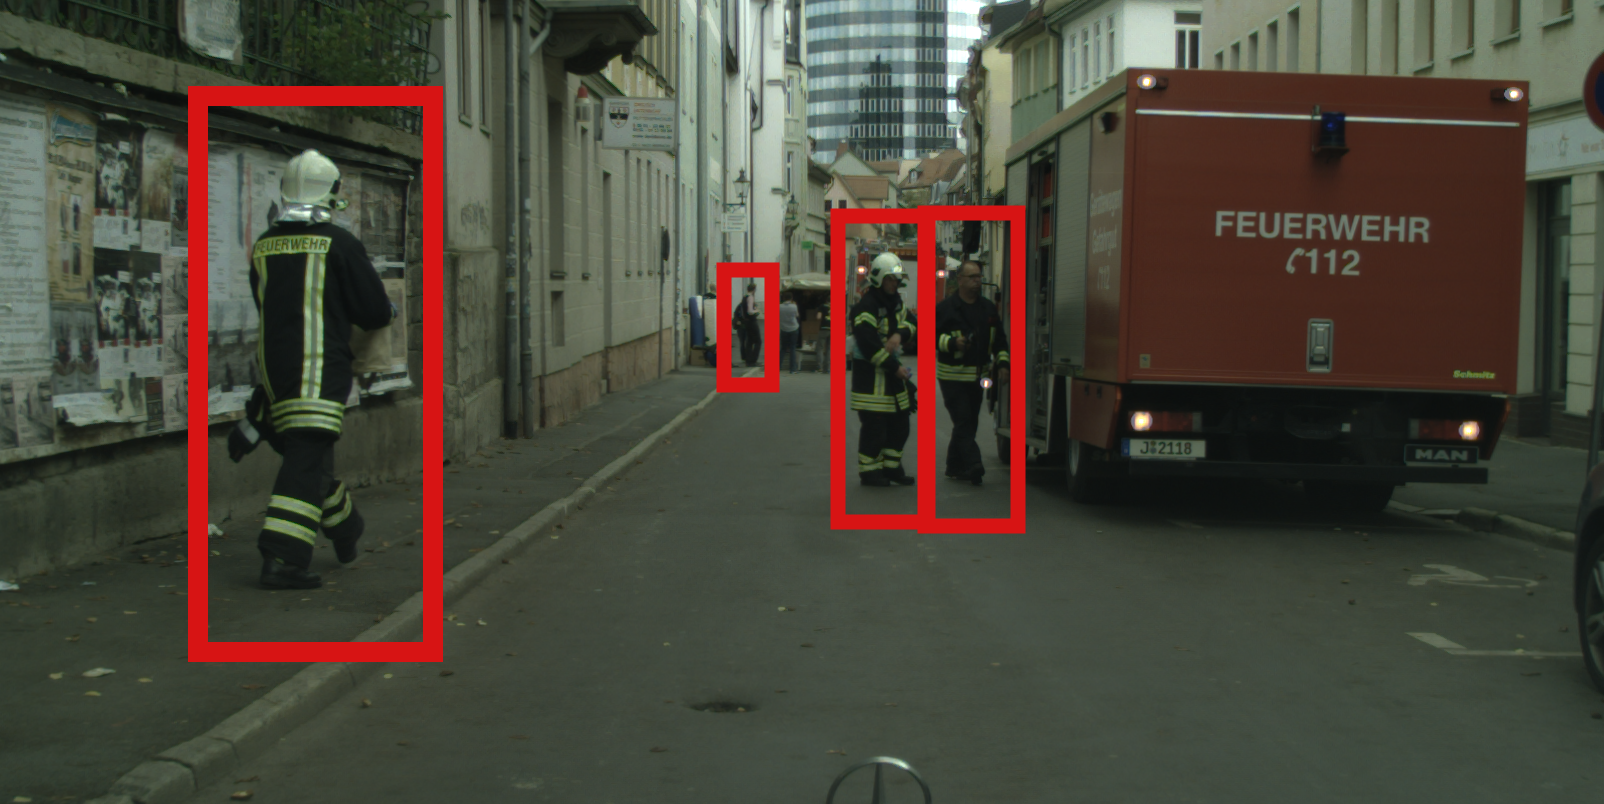
\includegraphics[width=\linewidth]{ekya/figures/motivation/incr_learn_motivation/t6_marked.png}
    % 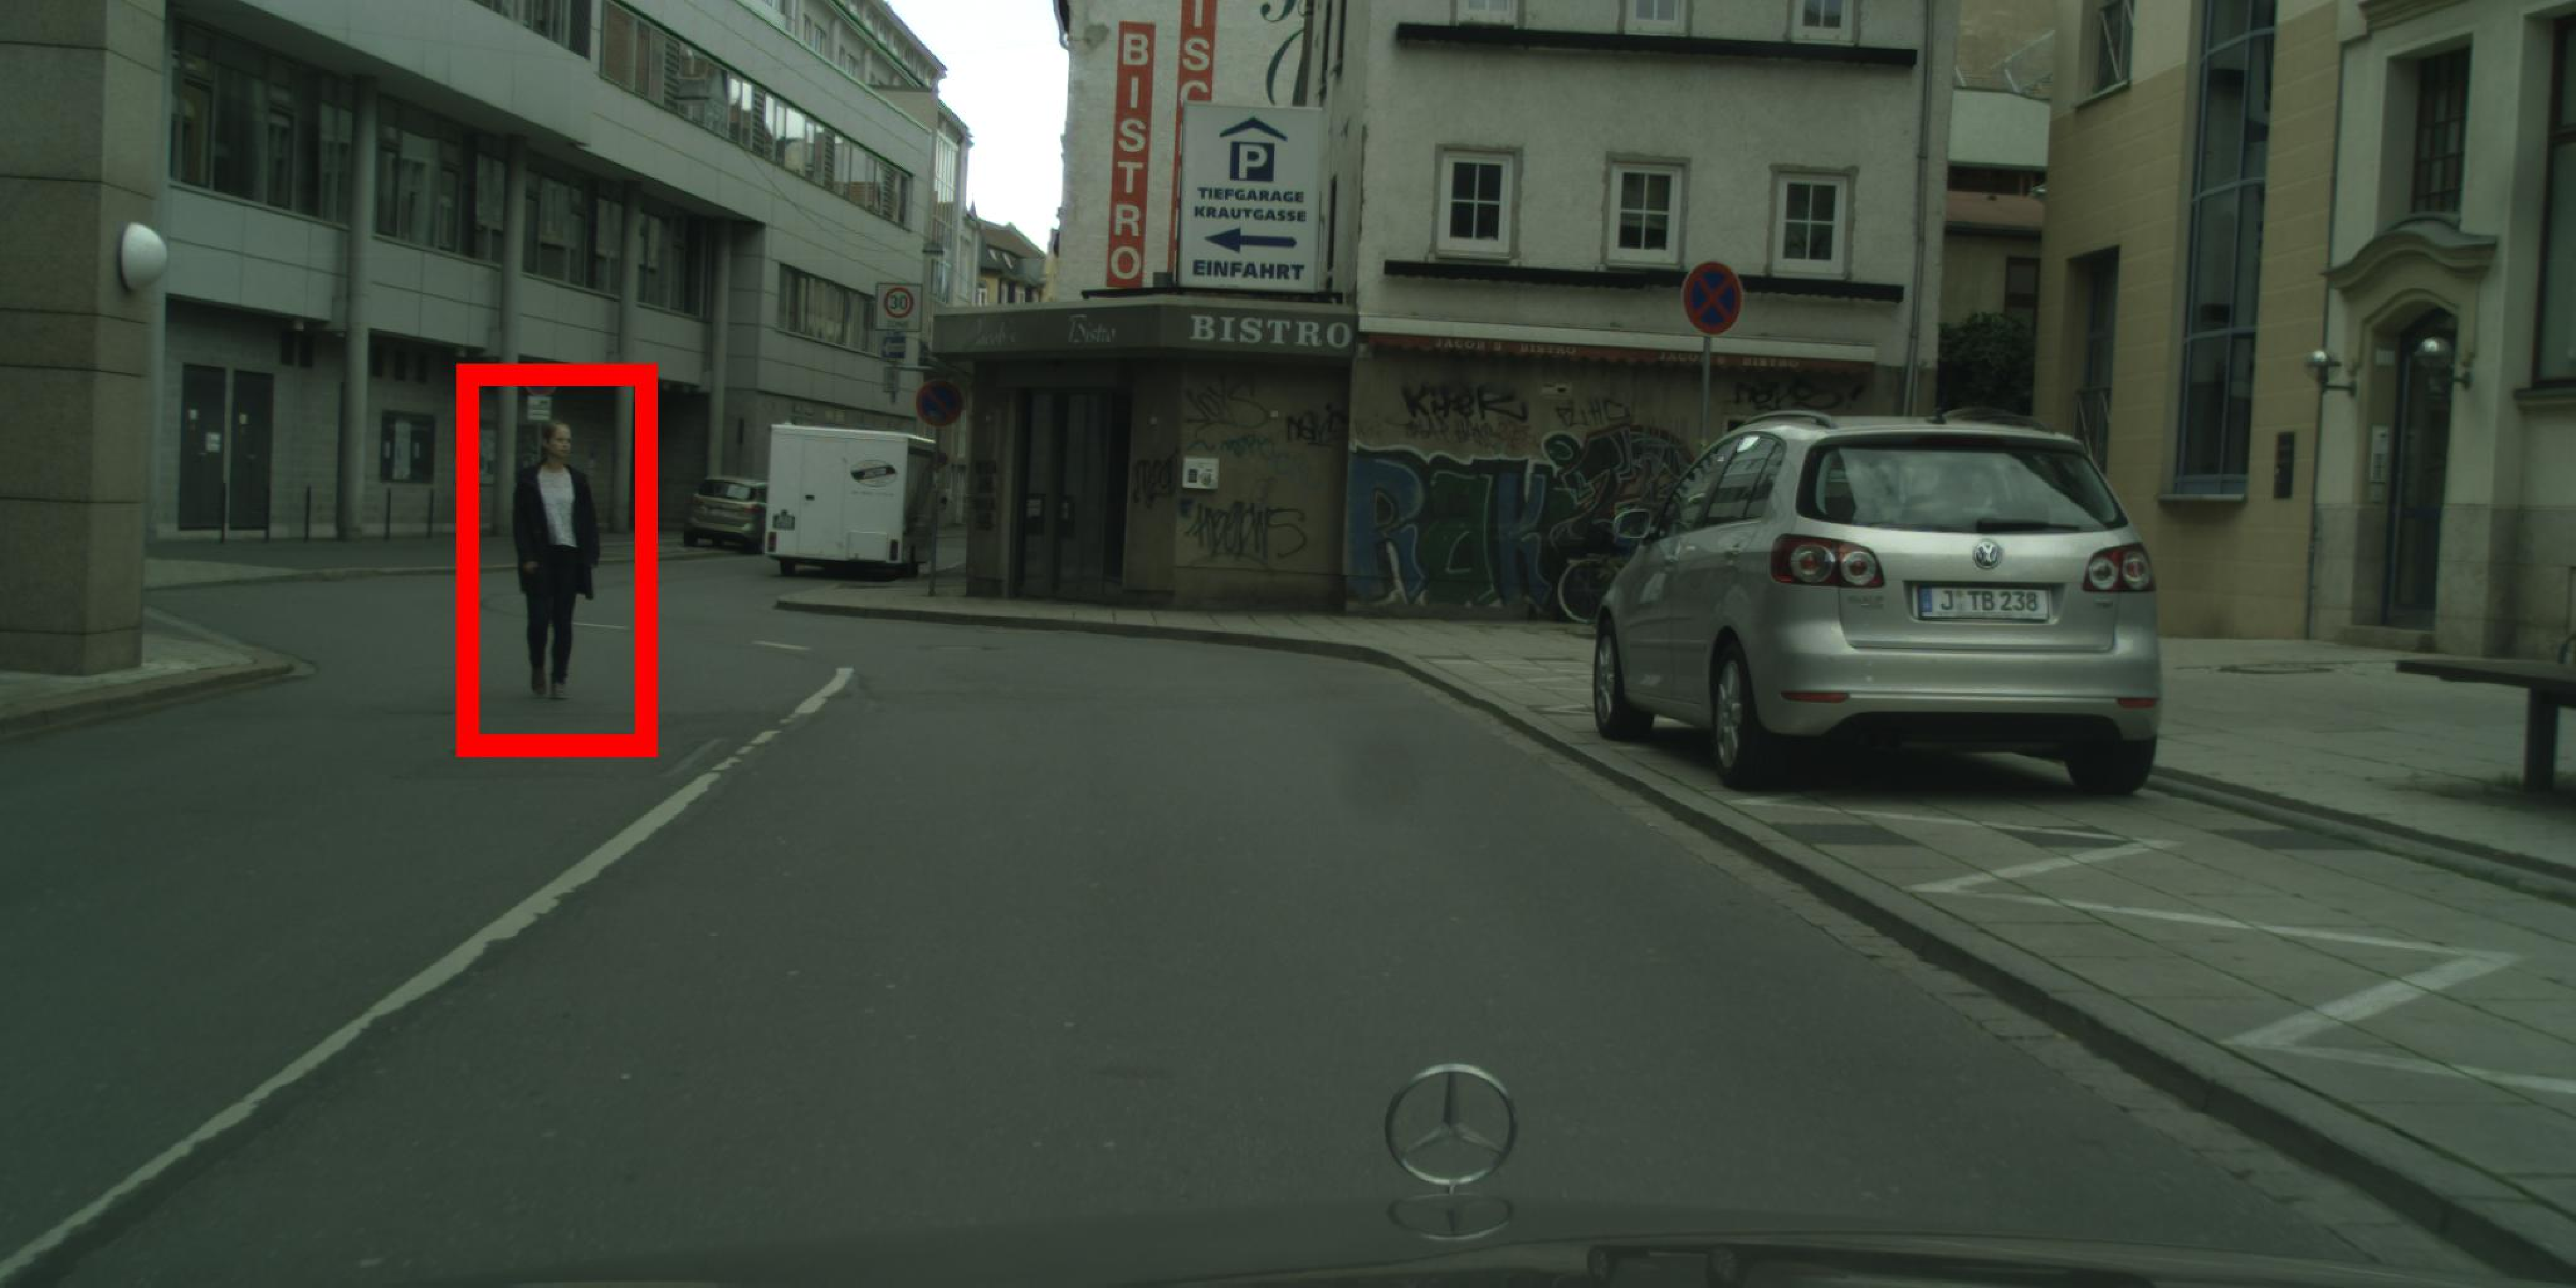
\includegraphics[width=\linewidth]{ekya/figures/motivation/incr_learn_motivation/motivation_cityscapes_jena_win5.pdf}
    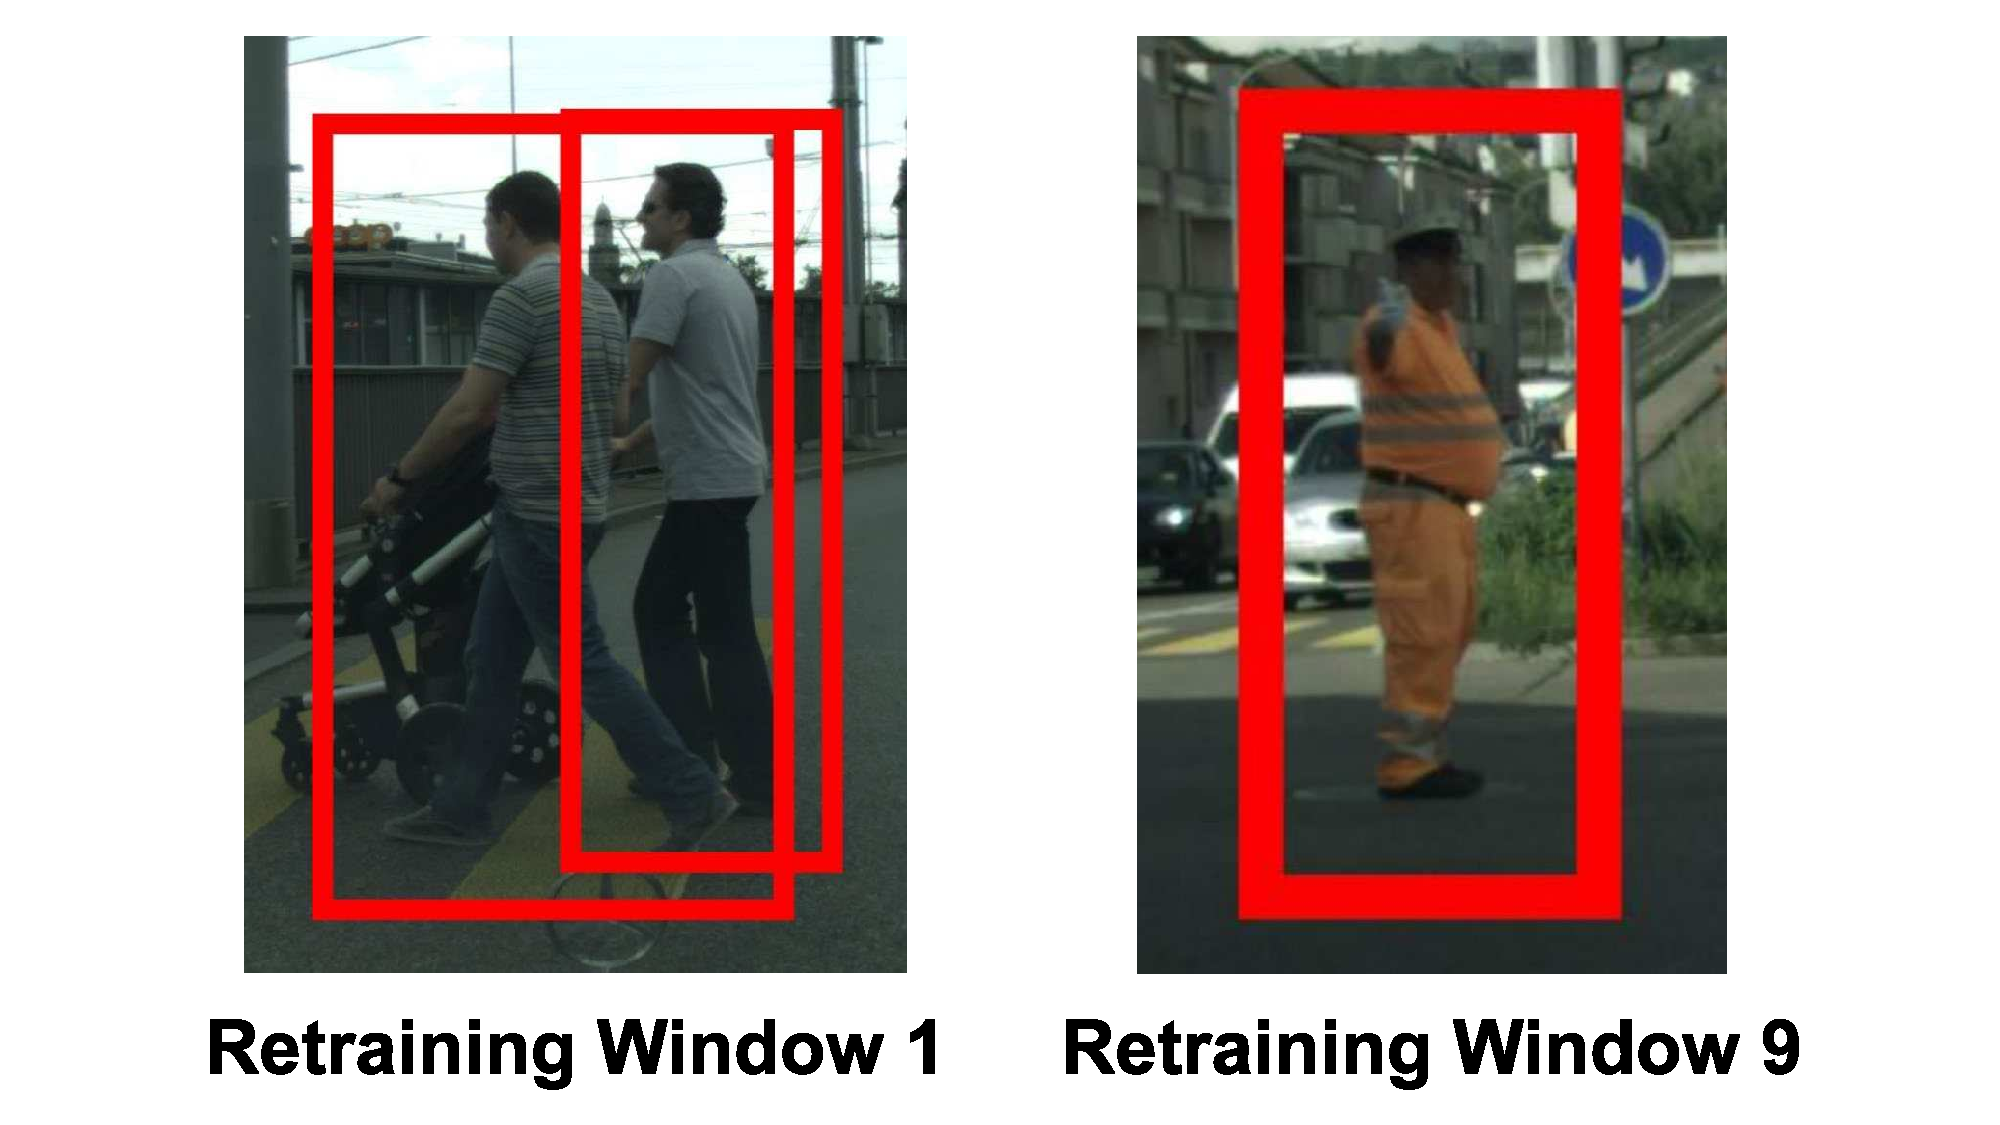
\includegraphics[width=\linewidth]{ekya/figures/motivation/incr_learn_motivation/person_classshift.pdf}
    \caption{\small Person class variations}
    \label{fig:personclass}
  \end{subfigure}
  
   \caption{\bf\small \cameratext{Continuous learning in the Cityscapes dataset. Shift in class distributions (a) across windows necessitates continuous learning (b). Model accuracy is not only affected by class distribution shifts (c), but also by changes in object appearances (d).}}% As more data samples are made available to model for retraining, it achieves a higher accuracy compared to a pre-trained model which does not adapt to the new data samples. We evaluate the accuracy of the following classes -- 'person', 'car, 'truck', 'bus', 'bicycle', 'motorcycle'.}
  \label{fig:cityscapes-motivation}
\end{figure}



%To show the benefits of continuous learning, we use two video datasets that were collected from dashboard cameras in cars: Cityscapes \cite{cityscapes} in Europe and Waymo \cite{waymo} in the USA. These cameras collect data samples over time and at different locations. (Details of the datasets in \S\ref{subsec:eval-setup}). 

To show the benefits of continuous learning, we use the video stream from one example city in the Cityscapes dataset \cite{cityscapes} that consists of videos from dashboard cameras in many cities. %over time and at different locations. 
In our evaluation in \S\ref{sec:evaluation}, we use both moving dashboard cameras as well as static cameras over long time periods. 
We divide the video data in our example city into ten fixed \emph{retraining windows} (200s in this example). 


\noindent\cameratext{\textbf{Understanding sources of data drift.} Figure \ref{fig:jena-classdist} shows the change of object class distributions across windows. The initial five windows see a fair amount of persons and bicycles, but bicycles rarely show up in windows 6 and 7, while the share of persons varies considerably across windows $6-10$. Figure~\ref{fig:acc-datadrift} summarizes the effect of this data drift on model accuracy in five independent video streams, C1-C5. For each stream, we train a baseline model on the first five windows, and test it against five windows in the future and use cosine similarity to measure the class distribution shift for each window. Though accuracy generally improves when the model is used on windows with similar class distributions (high cosine similarity), the relationship is not guaranteed (C2, C3). This is because class distribution shift is not the only form of data drift. Illumination, pose and appearance differences also affect model performance (e.g. clothing and angles for objects in the person class vary significantly; Figure \ref{fig:personclass}).}

\noindent\cameratext{\textbf{Improving accuracy with continuous learning.}} Figure \ref{fig:jena-motivation} plots inference accuracy of an edge DNN (a compressed ResNet18 classifier) in the last five windows using different training options. 
%: (1) pretrain the model with representative data from \kh{10} other cities in the same dataset; (2) pretrain the model with recent history (the first five windows) in the same video; and (3) continuously retrain the model in every window. 
%$(1)$ Starting with an off-the-shelf ResNet18 model that was trained on the ImageNet dataset \cite{DBLP:journals/ijcv/RussakovskyDSKS15} and further tuned 
$(1)$ Training a compressed ResNet18 with video data on all other cities of the Cityscapes dataset does not result in good performance.
%Note that tuning off-the-shelf models using related datasets is common in deployments. 
$(2)$ Unsurprisingly, we observe that training the edge DNN once using data from the first five windows {\em of this example city} improves the accuracy. %by $9\%$ on average. 
$(3)$ %However,  
%We observe that the pretrained model using all data from \kh{4} other cities performs poorly. Similarly, using data from the first five windows to pretrain the edge DNN also suffers from accuracy drops in the next five windows. Both results show the limitation of pretraining edge DNNs with large and representative data.  
%In contrast, 
{\em Continuous retraining} using the most recent data for training achieves the highest accuracy consistently. Its accuracy is higher than the other options %first two offline training options 
by up to $22\%$.%$ $15\%$ and $6\%$, respectively.  %and its accuracy is much higher and more consistent. 
%Its accuracy is up to \kh{$25\%$} higher than the pretrained DNNs in one window. On average across all windows, continuous retraining leads to \kh{$10\%$ to $20\%$} higher accuracy over the pretrained DNNs. 

\revtext{Interestingly, using the data from the first five windows to train the larger ResNet101 DNN (not graphed) achieves better accuracy than the continuously retrained ResNet18.}  %While this gap indicates the %presence of data drift and the 
%benefit of using the most recent data for training, 
The substantially better accuracy of ResNet101 compared to ResNet18 when trained {\em on the same data} of the first five windows also shows that this training data was indeed fairly representative. But the lightweight ResNet18's weights and architecture limits its ability to learn and is a key contributor to its lower accuracy.
%This shows that the data in the first five windows is in fact fairly representative, but the ResNet18 model's cheaper weights and architecture is a key factor contributing to its lower accuracy. 
Nonetheless, ResNet101 %is unsuited for live video inference as it takes $50-260$ms per inference on edge class GPUs \cite{cnn-perf}, which 
is $13\times$ slower than the compressed ResNet18 \cite{cnn-perf}. % which makes the latter more suited for edge deployments.
%cost of $50-260$ms per inference on edge class GPUs 
%. 
This makes the efficient ResNet18 more suited for edge deployments and continuous learning enables it to maintain high accuracy even with data drift. Therefore, the need for continuous training of edge DNNs is ongoing and not just during a ``ramp-up'' phase. %We use the even more expensive \gaa{ResNext101} as our golden model for labeling, and we have verified that its results almost match manual labeling.
% Efficiency between ResNet101 and ResNet18 Ref: https://github.com/jcjohnson/cnn-benchmarks
% Our measured 
% is unable to memorize all the data.



%even though the edge DNN is pretrained with \kh{10$\times$} of data samples from the same dataset.  
%As Figure \ref{fig:jena-classdist} shows, class distribution changes quickly over time. The initial training samples are dominated by vehicles, but a lot more pedestrians and motorcycles show up at later time. 
%The appearance of objects also changes significantly, such as pedestrians show up in different clothing and angles at different time (Figure \ref{fig:jena-image-1} and \ref{fig:jena-image-6}).
%Figure \ref{fig:jena-motivation} shows that such data shift causes major accuracy drop for edge DNNs (ResNet18 in this example) that are pretrained with data from other cities. 
%We also see considerable accuracy drop even when the edge DNN is retrained with the same video in the first one and first three windows.


%Retraining window $6$ in Figure \ref{fig:cityscapes-motivation} highlights an interesting aspect. The distributions of classes in window \kh{$6$} and window \kh{$1$} are similar (Figure \ref{fig:jena-classdist}), yet the continuously retrained model achieves much higher accuracy than the model that is pretrained with data in window \kh{$1$} (Figure \ref{fig:jena-motivation}). Visual inspection suggests that this difference is likely due to the varying appearance and angles of objects (e.g., people with different clothing) between the two windows; see Figures \ref{fig:jena-image-1} and \ref{fig:jena-image-6}.% Thus, continuous learning is valuable even when the class

%Figure \ref{fig:waymo-motivation-distrib} illustrates how class distribution and DNN inference accuracy change over time in one city in the Waymo dataset, and the results are shown in fixed \emph{retraining windows} (\kh{xx} seconds in this example). 
%As Figure \ref{fig:class-distrib-motivation} shows, class distribution changes significantly over time. The initial training samples are dominated by vehicles, but a lot more pedestrians and road signs show up at later time. 
%As Figure \ref{fig:class-distrib-motivation-acc} shows, this data shift causes major accuracy drop for edge DNNs (ResNet18 in this example) that are pretrained with offline data in the same dataset. 
%We also see considerable accuracy drop even when the edge DNN is retrained with the \emph{first half} of the video in this camera.
%In contrast, the continuously retrained DNN keeps using recent data to cope with the changing distributions, and it achieves \kh{$xx\%$ and $yy\%$} higher accuracy over the DNNs that are pretrained with the offline and first half video data, respectively. We observe similar phenomenon in all other cities in the Waymo dataset, as continuously retrained edge DNNs achieve \kh{xx\%} higher accuracy over pretrained edge DNNs on average (up to \kh{yy\%}). \footnote{In Figures \ref{fig:waymo-motivation-distrib} and \ref{fig:cityscapes-motivation}, at each retraining window $i$ on the x-axis, the data from ($i-2, i-1$) is used for retraining the model, and the data from ($i-1, i$) is used for inference (testing), whose accuracy in turn is plotted on the y-axis.}

%Figure \ref{fig:class-distrib-motivation} demonstrates the impact of changes to the distribution of object classes in (a single city of the Waymo data) on the ResNet18 classifier. We compare the accuracies of a continuously updated ResNet18 classifier against the version of ResNet18 that was pre-trained only once initially (on a few samples from this video). 
%Further, continuous learning is also beneficial when the {\em distribution} of data samples of the object classes changes over time; Figure \ref{fig:class-distrib-motivation}. 
%While the initial training samples are dominated by vehicles, more examples of pedestrians  and road signs become available with time (Figure \ref{fig:class-distrib-motivation}). This is typical of video data in suburban cities where the pedestrian traffic is considerably lower than vehicular traffic. The changing distribution causes the once-trained ResNet18's accuracy to drop while the continuously trained model keeps retraining itself with the recent data, copes with the changing distributions, and achieves $28\%$ higher accuracy (Figure \ref{fig:class-distrib-motivation-acc}). \footnote{In Figures \ref{fig:waymo-motivation-distrib} and \ref{fig:cityscapes-motivation}, at each retraining window $i$ on the x-axis, the data from ($i-2, i-1$) is used for retraining the model, and the data from ($i-1, i$) is used for inference (testing), whose accuracy in turn is plotted on the y-axis.}




% sample incremental; jena and tubingen of cityscapes
%Figure \ref{fig:cityscapes-motivation} shows the benefits of {\em sample-incremental} training, i.e., improving the model with newer data samples over time. %We use two videos for this experiments from cars driving in two cities, Jena and Tubingen. 
%We compare the accuracies of the continuously updated ResNet18 convolutional classifier against the version of ResNet18 that was trained only once initially (on a few representative samples before the edge model was deployed). 

%Figure \ref{fig:cityscapes-motivation} shows the similar phenomenon of the impact of changing class distributions (Figure \ref{fig:jena-classdist}) with the Cityscapes data (again, a single city). 
%As Figure \ref{fig:jena-motivation} shows, continuously retrained DNN achieves much higher (by \kh{$zz\%$}) and more steady accuracy than the pretrained DNNs.
%Across all cities in the Cityscapes dataset, continuously retrained DNNs achieve \kh{xx\%} higher accuracy over pretrained edge DNNs on average (up to \kh{yy\%} higher).
%while the accuracies of the two models -- continuously-trained and once-trained -- are similar at the beginning, over time, continuous learning leads to the model's accuracy being higher (by $27\%$) and relatively steady. % they diverge over time to a difference of as much as $27\%$ in accuracy. Continuous learning results in relatively steady (and higher) accuracy over time. %We observe a similar trend in Figure \ref{fig:tubingen-motivation} where the divergence in accuracy due to not updating the model is observed immediately. (Note that in each of Figure \ref{fig:jena-motivation} and \ref{fig:tubingen-motivation} our experiments use new data samples over time obtained from a {\em single} city.)  
%Retraining window $6$ in Figure \ref{fig:cityscapes-motivation} highlights an interesting aspect. The distributions of classes in window \kh{$6$} and window \kh{$1$} are similar (Figure \ref{fig:jena-classdist}), yet the continuously retrained model achieves much higher accuracy than the model that is pretrained with data in window \kh{$1$} (Figure \ref{fig:jena-motivation}). Visual inspection suggests that this difference is likely due to the varying appearance and angles of objects (e.g., people with different clothing) between the two windows; see Figures \ref{fig:jena-image-1} and \ref{fig:jena-image-6}.% Thus, continuous learning is valuable even when the class distributions are similar.

%%Comparing against a version of the model that is trained on representative data initially is conservative because typical deployments use off-the-shelf models that are pre-trained on standard datasets (e.g., ImageNet \cite{imagenet} or MS-COCO \cite{coco}). 
%%%%%Our experiments, overall, demonstrate the value of improving the models with new data samples to cope with changing data distributions as well as changing conditions and appearances of the objects. 
%\junchen{hmm.. i do see the point that having more samples helps, but in any event, people will use a model (even a cheap one) trained offline with some {\em large} standard dataset (imagenet, coco, etc). i tend to believe the gain is due to fine-tuning the ResNet model to in-situ data from the Cityscape ``scene'' and more such data the better?}
%%Continuous learning also helps to learn altogether new object classes, whose examples may not have been included in the training data \cite{incremental-24, icarl-14}.
%\noindent{\bf Rate of change.} Finally, different videos change at different rates. Urban settings typically observe higher change in their data distributions and will benefit from more frequent retraining, while suburban settings will do with a relatively lower retraining frequency. Likewise, times of busy traffic see a faster change in their data distributions compared to off-peak periods. In addition, the data distributions are also significantly different {\em across cities} (even if they are neighboring) in both the Waymo and Cityscapes datasets. Models that are deployed in vehicles moving across neighboring cities at different times will benefit from learning on new data. 

%We observe similar phenomenon across a diverse set of videos (see \S\ref{sec:evaluation}). Edge DNNs that are pretrained only once experience significant accuracy drop over time, even if their training data is from the same video in the recent history. These sharp accuracy drops make the inference results inconsistent and unreliable.  In contrast, continuous training enables edge DNNs to adapt with the most recent and relevant data, and it leads to much higher and more steady accuracy. 



%\begin{figure}[t!]
%  \centering
%  \begin{subfigure}[t]{0.5\linewidth}
%    \centering
%    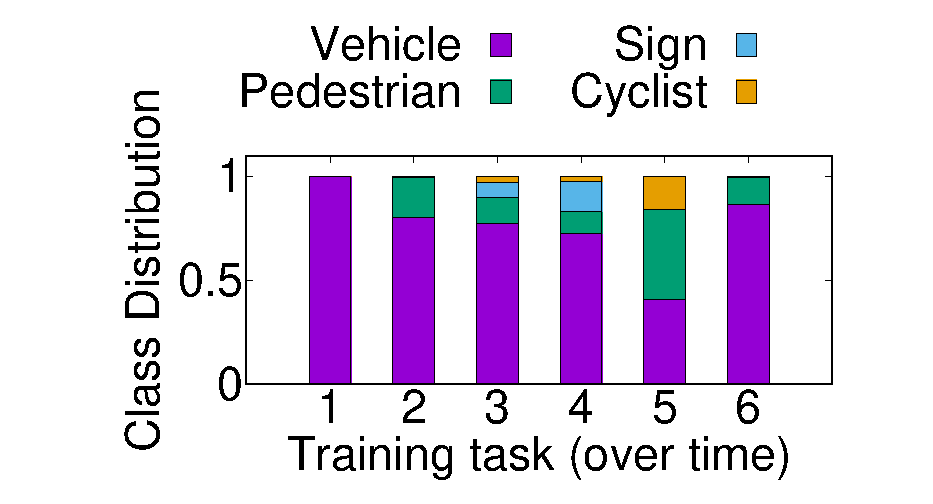
\includegraphics[width=\linewidth]{ekya/figures/motivation/Class_Incrementality/new_class.eps}
%    \caption{\small New classes over time}
%        \label{fig:class-inc-motivation}
%  \end{subfigure}
%  ~~
%  \begin{subfigure}[t]{0.5\linewidth}
%    \centering
%    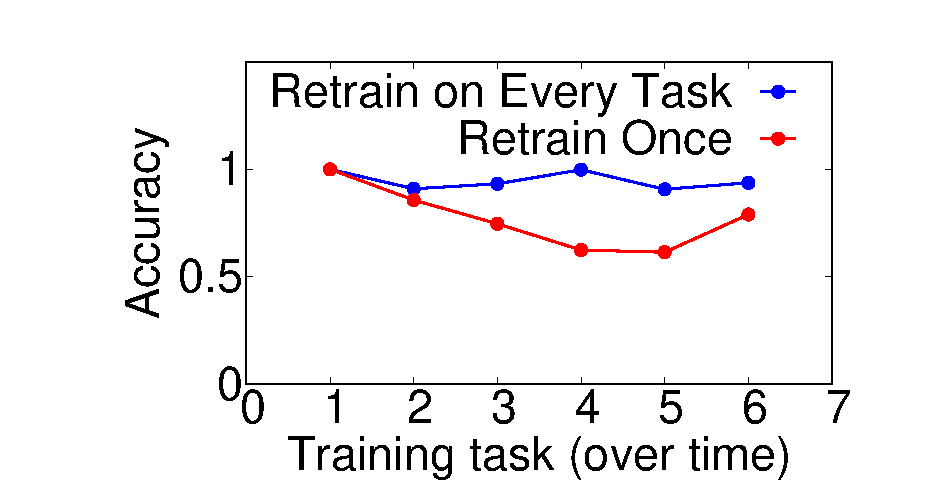
\includegraphics[width=\linewidth]{ekya/figures/motivation/Class_Incrementality/new_class_acc.eps}
%    \caption{\small Accuracy}
%        \label{fig:class-inc-motivation-acc}
%  \end{subfigure}
%   \hfill
%  ~~
%  \caption{\bf\small Class incremental learning with Waymo.}
%  \label{fig:waymo-motivation}
%\end{figure}

%{\em Class-incremental} training refers to learning new object classes with time, thus expanding the model's classification targets. As shown in Figure \ref{fig:class-inc-motivation}, the initial training data only consists of samples of vehicles, but over time, pedestrians, road signs, and cyclists are added. Continuously updating the ResNet18 model to include these new classes results in consistently higher accuracy by as much as $37\%$ (Figure \ref{fig:class-inc-motivation-acc}). \ion{This example is a bit contrived. Why would you even consider deploying a model for video traffic that is trained only on cars in the first place?}


% impact of different retraining frequencies - show variation across two cities
%\ga{TODO paragraph.} \textbf{Retraining Frequency.} As a model specializes for a specific data distribution, its performance on general data decreases.  Moreover, frequent retraining requires more resources, which may not be available and thus the model may be trained only for a shorter duration \romil{The inference-resource-opportunity-cost argument can also be put here, but is not reflected in the plots}. Thus, a high retraining frequency can reduce the model accuracy.
%\junchen{Is retraining too frequently lowers the accuracy because of more frames being dropped or because of retraining ending prematurely for lack of resource? if so, please make it explicit. i was confused as reader..}
%This is observed in \cref{fig:cologne-motivation} and \cref{fig:erfurt-motivation}, where having just 2 tasks \romil{Explain what a task is} has a mean accuracy of 70.4\% over the entire dataset, but decreases to 69.8\% when retrained over 10 tasks. Similar behavior for Erfurt (82.9\% vs 82.2\%). 


% golden model; can retain more info but is expensive; edge model's capacity is less but is cheaper to execute
% show graph - golden, edge w/ retraining, edge w/o retraining (for one of the above cities); both sample and class incremental
% romilb: a third line in figure 1 - (showing continuously high accuracy?) 

%\noindent{\bf Golden model.}



% used for inference already; we propose running training too; storage isn't a concern but compute is limited; the network is also a worry, so we cannot access the infinite compute in the cloud
%\subsection{\bf Joint inference and retraining on edge servers.}
%Our proposal is to extend the edge servers, which already performs video DNN inferences, to {\em include continuous training of the edge DNN models}. Edge servers already have capacity to store the limited amount of recent video data that is required for continuous retraining. However, its compute capacity is a concern as the edge server's compute is already provisioned for the DNN inference on live video streams. Since retraining is periodic, i.e., its compute requirements are bursty in nature, provisioning compute resources for retraining will lead to wasted utilization and increased cost (by as much as \gaa{XXX} in our experiments). For the reasons explained in \S\ref{subsec:edge} regarding bandwidth constraints and privacy sensitivities, transmitting the videos to the cloud for retraining is not preferred. 
%As we describe next, we develop techniques to minimize disruption to the inference while smartly allocating resources for continuous retraining. %maximize the eventual inference accuracy. 

